\section{Background}

\subsection{Time series}
% TODO add hearth observation example 
A time series is a sequence of observations taken at regular intervals of time.
These observations can be numerical values, categorical variables, or even text.
Time series data is commonly found in a wide range of fields such as finance, economics, healthcare, meteorology, and transportation.

\begin{figure}[h]
  \centering
  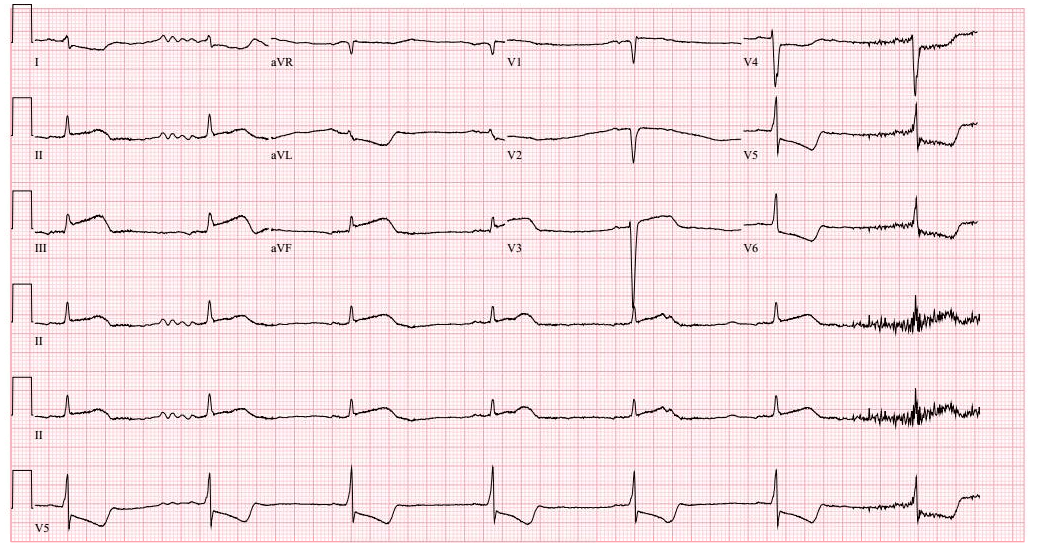
\includegraphics[width=0.45\textwidth]{timeseries-ex1}
  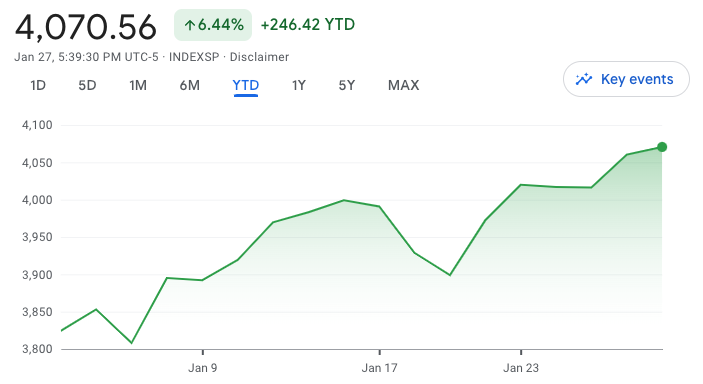
\includegraphics[width=0.45\textwidth]{timeseries-ex2}
  \caption{Example of timeseries data}
\end{figure}

In finance, for example, time series data can be used to analyze stock prices, interest rates, and currency exchange rates.
In healthcare, time series data can be used to analyze patient vital signs, such as heart rate and blood pressure.
In transportation, time series data can be used to analyze traffic patterns and traffic flow.
% TODO add hearth observation example


% TODO talk about this too?
% There are several characteristics that define a time series, including:
% Regular time intervals: Observations are taken at regular intervals of time, such as every minute, hour, day, or month.
% Ordering: The observations are ordered in time, meaning that the observation at time t is followed by the observation at time t+1.
% Time dependence: The value of the observation at time t is dependent on the values of the observations at previous time steps.
% Stationarity: A time series is considered stationary if its statistical properties, such as mean and variance, do not change over time.
% One of the main challenges in working with time series data is the presence of missing values. This can occur due to various reasons such as sensor failures, data transmission errors, or data cleaning processes. The presence of missing values can make it difficult to perform tasks such as classification and prediction on time series data.
\subsubsection[short]{Univariate and Multivariate}

In addition to the concept of a time series, it's also important to understand the difference between univariate and multivariate time series.
\begin{figure}[h]
  \centering
  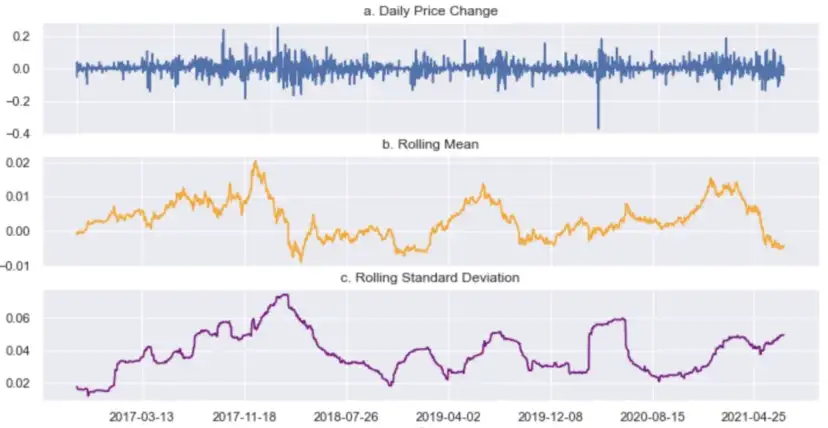
\includegraphics[width=0.6\textwidth]{multivariate}
  \caption{Example of Multivariate timeserie}
\end{figure}

\paragraph{Univariate time series:} This type of time series includes observations of a single variable, such as stock prices or temperature. The main focus is on understanding the patterns and trends in the single variable over time.
\paragraph{Multivariate time series:} This type of time series includes observations of multiple variables, also known as features, over time. The main focus is on understanding the relationships and interactions between the multiple variables.

In univariate time series, the focus is on understanding the patterns and trends of a single variable over time. This can be done by analyzing the data using techniques such as time series decomposition, trend analysis, and forecasting.
On the other hand, in multivariate time series, the focus is on understanding the relationships and interactions between multiple variables. 
%Techniques such as vector autoregression (VAR) and principal component analysis (PCA) can be used to analyze the relationships between the variables. Additionally, multivariate time series can also be used for tasks such as classification and anomaly detection.
It's important to note that, the choice of model and the methods used to analyze the data will depend on the type of time series data you are working with. Univariate and multivariate time series require different approach and techniques to be analyzed.

\subsubsection[short]{Spatio-temporal autocorrelation}
Spatio-temporal autocorrelation refers to the correlation between observations that are close in both space and time. It is a common phenomenon in many natural and social phenomena, such as weather patterns, crime rates, and population density.

Spatio-temporal autocorrelation can be of two types: positive and negative. Positive spatio-temporal autocorrelation occurs when similar values tend to cluster together in both space and time. For example, in weather patterns, regions with high temperatures tend to be near other regions with high temperatures, and this pattern tends to persist over time. Negative spatio-temporal autocorrelation occurs when dissimilar values tend to cluster together in both space and time.

Spatio-temporal autocorrelation is important to consider when analyzing spatio-temporal data, such as time series data with a spatial component. Ignoring spatio-temporal autocorrelation can lead to biased and unreliable results.

\subsection{Ensemble learning}
Ensemble learning is a technique in machine learning where multiple models are combined to create a more powerful model. The idea behind ensemble learning is that by combining the predictions of multiple models, the ensemble model can reduce the variance and bias of the individual models, leading to improved performance on unseen data.

There are several popular ensemble learning methods, including:

\paragraph{Bagging:}This method involves training multiple models independently on different subsets of the data, and then combining their predictions through a majority vote or averaging.

\paragraph{Boosting:} This method involves training multiple models sequentially, where each model tries to correct the mistakes of the previous model. The final predictions are made by combining the predictions of all the models.

\paragraph{Random Forest:} This method is a combination of bagging and decision trees. It involves training multiple decision trees independently on different subsets of the data, and then combining their predictions through a majority vote.

\paragraph{Stacking:} This method involves training multiple models independently and then using the predictions of these models as input features to train a meta-model.

Ensemble learning can be applied to a wide range of machine learning tasks, including classification, regression, and anomaly detection. It has been shown to improve performance on a wide range of datasets and is often used in practice to improve the performance of machine learning models.


\subsubsection{Random forests}

Random forests are an ensemble learning method used for classification and regression tasks. The name "random forest" comes from the fact that it is a collection of decision trees, where each tree is "trained" on a random subset of the data, and the final predictions are made by combining the predictions of all the trees.

\begin{figure}[h]
  \centering
  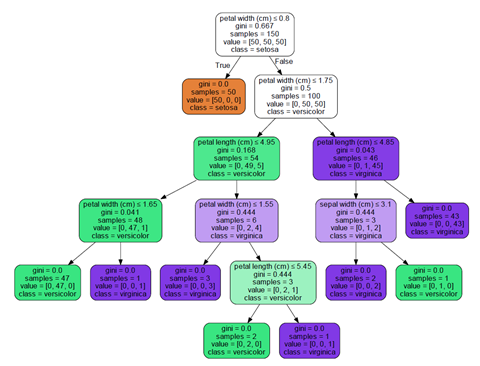
\includegraphics[width=0.8\textwidth]{decision-tree}
  \caption{Visual representation of a decision tree}
\end{figure}

A decision tree is a tree-like model that starts with a single node, called the root node, and splits the data into different subsets based on the values of the input features. Each internal node of the tree represents a test on an input feature, and each leaf node represents a prediction. The tree is built by recursively splitting the data until a stopping criterion is met, such as a maximum tree depth or a minimum number of samples in a leaf node.

In a random forest, multiple decision trees are trained on different subsets of the data, where the subsets are obtained by randomly sampling the data with replacement, also known as bootstrapping. Each tree is trained on a different subset of the data, and a different subset of the input features is used at each split of the tree. This is known as feature bagging or random subspace method.

When making a prediction, a random forest takes the average of the predictions of all the trees for regression problems, and takes a majority vote for classification problems. This combination of multiple decision trees reduces the variance of the individual trees and leads to improved performance on unseen data.

In summary, Random Forests are a combination of decision trees, where each tree is trained on a random subset of the data, and the final predictions are made by combining the predictions of all the trees. This combination of multiple decision trees reduces the variance of the individual trees and leads to improved performance on unseen data.



\subsection{Deep learning}
Deep learning is a subfield of machine learning that utilizes deep neural networks, which are neural networks with multiple hidden layers, to learn from the data.
These models are capable of learning abstract features from the data and making predictions based on those features, making them particularly useful for tasks such as image and speech recognition, natural language processing, and anomaly detection.

Deep neural networks are inspired by the structure and function of the human brain, consisting of layers of interconnected nodes, also known as neurons.
The input is passed through the layers of neurons, and the output is produced at the last layer.
The layers of a neural network can be divided into three main types: the input layer, the hidden layers and the output layer.
The input layer receives the input data, and the hidden layers perform computations on the data and pass the results to the next layer. 
The output layer produces the final predictions.

Deep learning models are trained using large amounts of data and powerful computational resources, such as GPUs.
The training process involves adjusting the parameters of the model, also known as weights, to minimize the error between the predictions and the true values.
This process is known as supervised learning, where the model learns to map inputs to outputs based on labeled examples.

In recent years, deep learning has made significant advancements in various fields, including computer vision, natural language processing, and speech recognition.
The ability of deep neural networks to learn abstract features has led to significant improvements in performance on various tasks, surpassing traditional machine learning methods.

In summary, deep learning is a subfield of machine learning that utilizes deep neural networks, which are neural networks with multiple hidden layers, to model complex patterns in data.
These models are trained using large amounts of data and powerful computational resources to minimize the error between predictions and true values and have led to significant advancements in various fields.

\subsubsection{Multilayer perceptrons}

Multilayer perceptrons (MLPs) are a popular class of feedforward artificial neural networks that are composed of multiple layers of artificial neurons.
These networks are also known as fully connected networks due to the fact that each neuron in one layer is connected to all neurons in the following layer.

\begin{figure}[h]
  \centering
  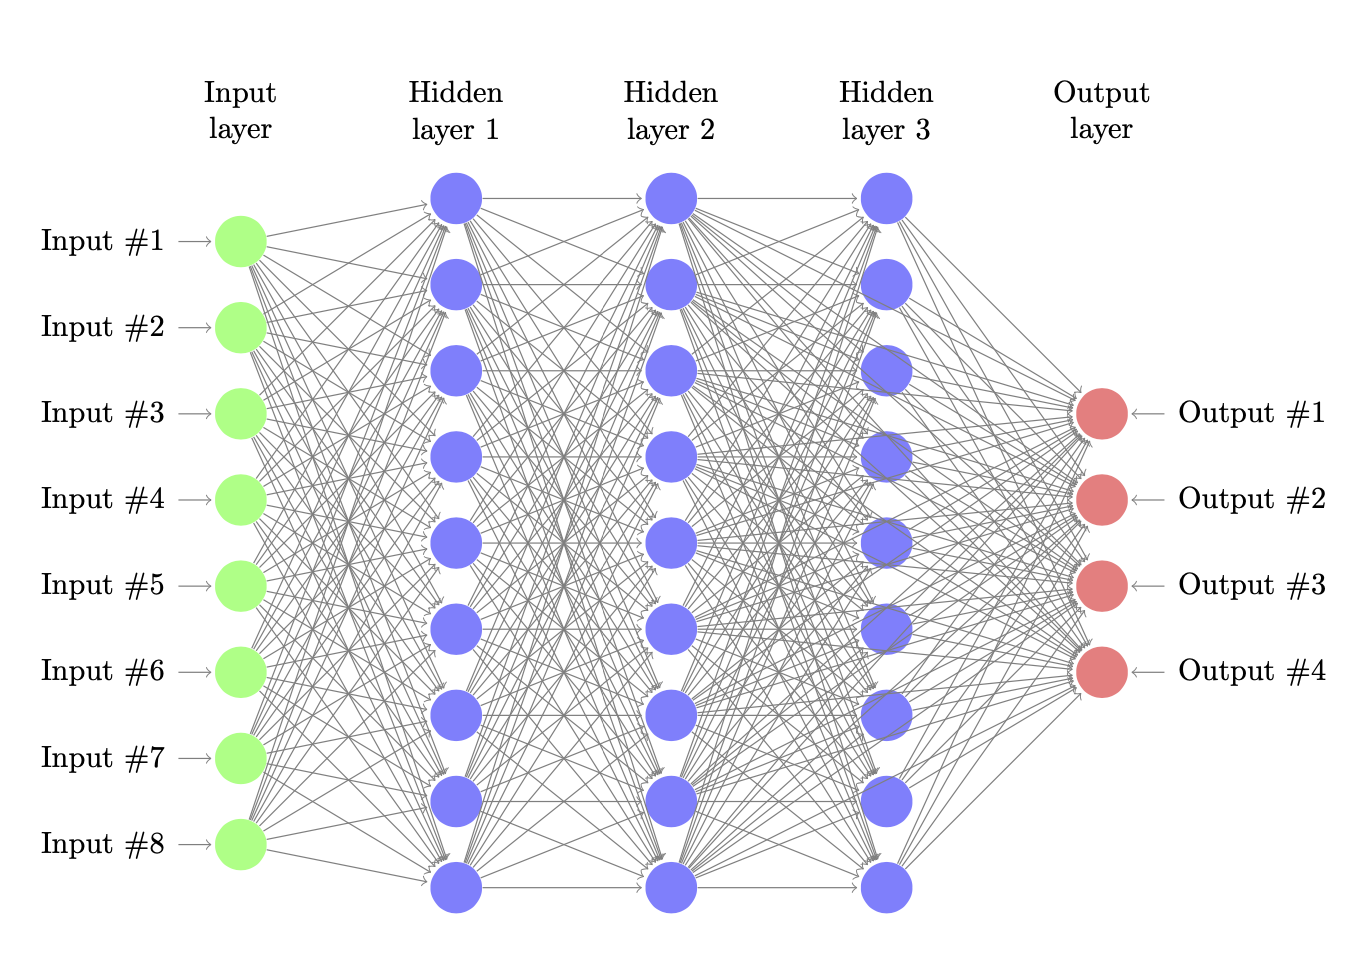
\includegraphics[width=0.8\textwidth]{mlp}
  \caption{Multilayer Perceptron (MLP) Diagram}
\end{figure}

% TODO explain more?
The perceptron is a single layer neural network that was first introduced by Frank Rosenblatt in 1957. 
It comprises of a single layer of artificial neurons, commonly referred to as perceptrons, which take in input and produce output. A perceptron is a linear classifier that separates the input data into two classes by using a linear decision boundary.

% TODO explain more?
\paragraph{Backpropagation} is the primary method used to train a multilayer perceptron. It is a supervised learning technique that utilizes the gradient descent optimization algorithm to adjust the weights of the network in order to minimize the error between the predicted output and the true output. The error is calculated using a loss function and is then propagated backwards through the network, adjusting the weights to reduce the error.

\paragraph {The learning rate} is a hyperparameter that controls the step size of the gradient descent optimization algorithm. It determines the extent to which the weights of the network should be adjusted in response to the error. A high learning rate results in larger weight adjustments, while a low learning rate results in smaller weight adjustments.

\paragraph {Overfitting} is a prevalent issue in neural networks and occurs when a model is trained too well on the training data, leading to poor performance on new, unseen data. To mitigate overfitting, techniques such as regularization and dropout can be employed.

\paragraph {Regularization} is a technique that adds a penalty term to the loss function, aimed at discourages the model from fitting to the noise in the training data. Common regularization methods include L1 and L2 regularization.

\paragraph {Dropout} is a technique that randomly drops out neurons during the training process, which helps to prevent overfitting by ensuring that no single neuron can have too much influence on the final predictions.

% TODO explain why
\paragraph{Activation functions} are utilized to introduce non-linearity into the network. They are applied to the output of each neuron before it is passed on to the next layer. Common activation functions include sigmoid, ReLU, and tanh.

In conclusion, Multilayer perceptrons (MLPs) are a popular class of feedforward artificial neural networks that are composed of multiple layers of artificial neurons.
The primary method used to train MLPs is backpropagation, which utilizes the gradient descent optimization algorithm to adjust the weights of the network.
To avoid overfitting, techniques such as regularization and dropout can be employed.
Activation functions are utilized to introduce non-linearity into the network.



\subsubsection{Convolutional neural networks}
Convolutional Neural Networks (CNNs) are a class of deep neural networks that are specifically designed to process data that has a grid-like structure, such as images.
CNNs are composed of multiple layers, including convolutional layers, pooling layers, and fully connected layers.


\begin{figure}[h]
  \centering
  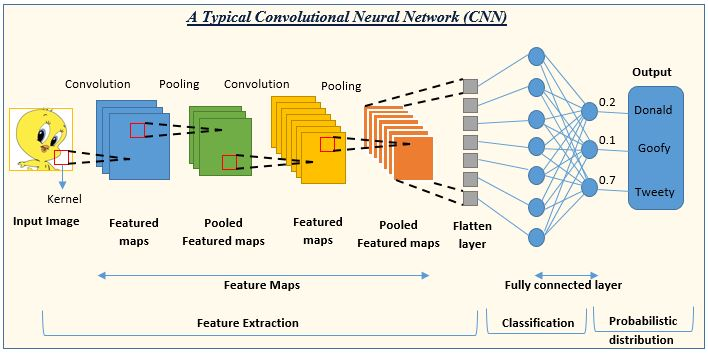
\includegraphics[width=0.8\textwidth]{cnn}
  \caption{Convolutional Neural Network (CNN) Diagram: A visual representation of a deep learning architecture consisting of layers of convolutional, pooling and fully connected layers.}
\end{figure}

% TODO explain better
The convolutional layer is the core component of a CNN.
It applies a set of learnable filters to the input data, which are used to extract features from the data.
These filters are convolved with the input data, resulting in a set of feature maps.
These feature maps are then passed on to the next layer for further processing.

Pooling layers are used to reduce the dimensionality of the feature maps and extract the most important features to increase the robustness of the network.
Max pooling and average pooling are two types of pooling layers that are commonly used. 

\begin{figure}[h]
  \centering
  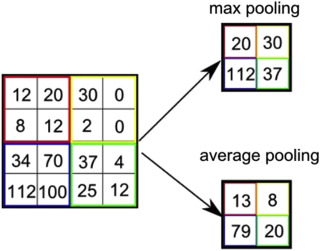
\includegraphics[width=0.4\textwidth]{pooling}
  \caption{Visualization of max and average pooling layers}
\end{figure}

Max pooling selects the maximum value from a small region of the input data. This operation is used to capture the most important feature in the region, such as the strongest edge or the highest intensity value. Max pooling is often used in image recognition tasks, as it is able to extract the most salient features from the input image, such as edges and textures.

Average pooling, on the other hand, takes the average value from a small region of the input data. This operation is used to reduce noise and smooth out small variations in the input data. Average pooling is often used in tasks such as image segmentation, as it is able to extract more subtle features from the input image, such as shapes and textures.

They both have different advantages and they are used in different tasks. Many CNNs use both max and average pooling in different layers.


Fully connected layers are used to classify the features extracted by the convolutional layers.
They take the output of the pooling layers and use it as input to a traditional feedforward neural network, which makes the final prediction.

CNNs have been successful in a wide range of image classification tasks and have been used to achieve state-of-the-art performance on benchmarks such as the ImageNet dataset.
They have also been applied to other domains, such as video analysis and natural language processing.

One of the key advantages of CNNs is their ability to learn spatially hierarchical representations of the data.
By using convolutional layers, CNNs can learn local patterns of the data and then compose these local patterns to form more complex patterns.
This is in contrast to traditional feedforward neural networks, which use fully connected layers and are not able to take advantage of the spatial structure of the data.

Another advantage of CNNs is their ability to learn translations-invariant representations of the data.
By using pooling layers, CNNs can learn representations that are robust to small translations of the input data.
This is important for tasks such as image classification, where the object of interest can be in different locations within the image.

In conclusion, Convolutional Neural Networks (CNNs) are a class of deep neural networks that are specifically designed to process data that has a grid-like structure, such as images.
CNNs are composed of multiple layers, including convolutional layers, pooling layers, and fully connected layers.
CNNs have been successful in a wide range of image classification tasks and have been used to achieve state-of-the-art performance on benchmarks such as the ImageNet dataset.
They have also been applied to other domains, such as video analysis and natural language processing.
CNNs are able to learn spatially hierarchical representations of the data and learn translations-invariant representations of the data.

\subsubsection{Temporal convolutional neural networks}

Temporal Convolutional Networks (TCNs) are a variation of CNNs that are designed to process sequential data, such as time series or videos.
They are similar to traditional CNNs in that they use convolutional layers to extract features from the input data, but they also incorporate temporal information by using dilated convolutions.

Dilated convolutions are similar to standard convolutions, but they have a dilation factor that controls the spacing between the elements of the convolutional kernel.
This allows TCNs to increase the receptive field of the network without increasing the number of parameters.
The result is that TCNs can capture long-term dependencies in the input data.

TCNs also use a causal convolution, which means that the output of the network only depends on the past inputs.
This is important in tasks such as prediction, where the future cannot be influenced by the current output.

TCNs have been used in a variety of tasks, such as speech recognition, natural language processing, and time series forecasting.
They have been shown to be effective in capturing temporal dependencies and have achieved state-of-the-art performance on benchmarks such as the Wall Street Journal corpus for speech recognition.

In conclusion, Temporal Convolutional Networks (TCNs) are a variation of CNNs that are designed to process sequential data, such as time series or videos.
They incorporate temporal information by using dilated convolutions and causal convolution which allows TCNs to increase the receptive field of the network without increasing the number of parameters and capture long-term dependencies in the input data.
TCNs have been used in a variety of tasks and have been shown to be effective in capturing temporal dependencies and have achieved state-of-the-art performance on benchmarks.


\subsubsection{Recurrent neural networks}

Recurrent Neural Networks (RNNs) are a type of neural network that are designed to process sequential data, such as time series or natural language.
They are called "recurrent" because they have a feedback loop that allows information to flow from one step of the sequence to the next.

RNNs have a hidden state, which is a vector that contains information about the past inputs.
At each time step, the input is combined with the hidden state to produce a new hidden state and an output.
The hidden state is then used as input for the next time step.

One of the main limitations of traditional RNNs is the vanishing gradient problem, which occurs when the gradients of the parameters tend to decrease exponentially with the number of time steps.
This makes it difficult to train RNNs on long sequences.
To overcome this problem, variants of RNNs have been developed, such as Long Short-Term Memory (LSTM) and Gated Recurrent Unit (GRU).

LSTMs and GRUs are architectures that introduce gates that control the flow of information through the hidden state, which allows them to remember information for longer periods of time. 

The main difference between LSTMs and GRUs is the number and complexity of the gates that they use to control the flow of information.
LSTMs use three gates: an input gate, an output gate, and a forget gate.
The input gate controls the flow of new information into the cell, the output gate controls the flow of information out of the cell, and the forget gate controls the flow of information through the cell.

GRUs, on the other hand, use two gates: an update gate and a reset gate.
The update gate controls the flow of new information into the cell, and the reset gate controls the flow of information through the cell.
The update gate can be seen as a combination of the input gate and forget gate in LSTM.

\begin{figure}[h]
  \centering
  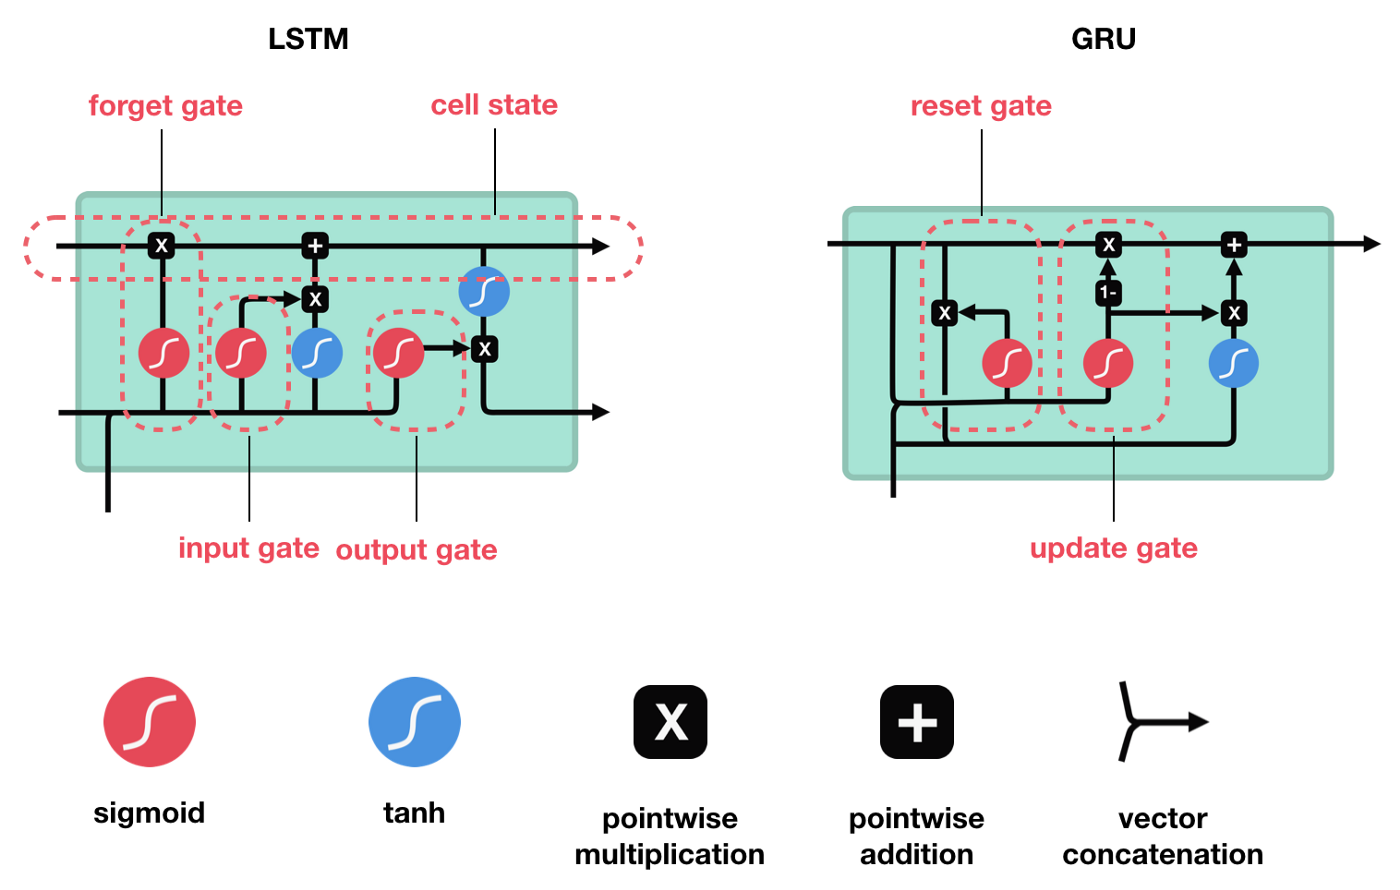
\includegraphics[width=0.6\textwidth]{lstm-gru}
  \caption{Visualization of LSTM and GRU cells}
\end{figure}

In terms of performance, both LSTMs and GRUs have been shown to be effective at handling long-term dependencies in sequential data.
LSTMs have been used in a wide range of applications such as language modeling, speech recognition, and machine translation, and have been shown to achieve state-of-the-art performance in many tasks.
GRUs, on the other hand, are more computationally efficient and have been used in applications such as natural language processing and speech recognition, and have been shown to achieve similar performance to LSTMs with fewer parameters.

In conclusion, Recurrent Neural Networks (RNNs) are a type of neural network that are designed to process sequential data.
They have a feedback loop that allows information to flow from one step of the sequence to the next and a hidden state that contains information about the past inputs.
However, traditional RNNs suffer from the vanishing gradient problem, which makes it difficult to train RNNs on long sequences.
To overcome this problem, variants of RNNs such as Long Short-Term Memory (LSTM) and Gated Recurrent Unit (GRU) have been developed. Both LSTMs and GRUs have been shown to be effective in solving a wide range of problems related to sequential data and have been applied to other areas as well.

\subsubsection{Generative adversarial networks}
- Generator

- Discriminator

Generative Adversarial Networks (GANs) are a type of neural network architecture that is used for unsupervised learning. They consist of two main components: a generator network and a discriminator network. The generator network is trained to generate new data samples that are similar to a given training dataset, while the discriminator network is trained to distinguish between the generated samples and the real samples from the training dataset.

The training process of GANs is based on a game-theoretic approach, where the generator and the discriminator are competing against each other. The generator is trying to generate samples that are similar to the real samples, while the discriminator is trying to correctly identify which samples are real and which are generated. As the training progresses, the generator becomes better at generating realistic samples, while the discriminator becomes better at identifying the generated samples.

One of the main advantages of GANs is that they can be used to generate high-quality images, videos, and other types of data. They have been used in a wide range of applications, including image synthesis, image-to-image translation, style transfer, and video prediction. GANs have also been applied to other areas such as natural language processing, speech synthesis, and 3D object generation.

There are many variations of GANs, such as Wasserstein GANs, which use the Wasserstein distance to measure the difference between the generated samples and the real samples, and Cycle GANs, which are used for image-to-image translation. There are also GANs that use different architectures, such as convolutional GANs and recurrent GANs.

Conditional GANs, also known as cGANs, are a variant of GANs where both the generator and the discriminator are conditioned on some additional input, such as a class label or an image. This allows the model to generate new samples that are conditioned on a specific class or attributes. For example, it can generate images of a specific object or in a specific style.

In conclusion, Generative Adversarial Networks (GANs) are a type of neural network architecture that is used for unsupervised learning. They consist of two main components: a generator network and a discriminator network. The generator network is trained to generate new data samples that are similar to a given training dataset, while the discriminator network is trained to distinguish between the generated samples and the real samples from the training dataset. GANs have many advantages, such as the ability to generate high-quality images, videos, and other types of data. Conditional GANs are a variant of GANs where both the generator and the discriminator are conditioned on some additional input, such as a class label or an image, allowing the model to generate new samples that are conditioned on a specific class or attributes. They have been used in a wide range of applications and have been applied to other areas such as natural language processing, speech synthesis, and 3D object generation

\subsubsection{Attention is all you need}
- Transformer
The "Attention is All You Need" (AIAYN) model, also known as the Transformer, is a neural network architecture that was introduced in 2017 by Google researchers. It is a type of encoder-decoder model that is primarily used for natural language processing tasks such as language translation, text summarization, and question answering.

The key innovation of the Transformer is the use of self-attention mechanisms, which allow the model to focus on specific parts of the input while processing it. Traditional encoder-decoder models use recurrent neural networks (RNNs) or convolutional neural networks (CNNs) to process the input sequentially, which can be slow and computationally expensive for long sequences. In contrast, the Transformer uses self-attention mechanisms to simultaneously process all parts of the input, which makes it much faster and more efficient.

The Transformer architecture consists of an encoder and a decoder, which are both made up of multiple layers of self-attention and feed-forward neural networks. The encoder takes in the input sequence and processes it using self-attention mechanisms, which allow the model to learn relationships between different parts of the input. The decoder then takes the encoded representation and generates the output sequence.

The attention mechanism used in the Transformer is a type of dot-product attention, which calculates the similarity between different parts of the input. The attention weights are then used to combine the different parts of the input to create a new representation.

One of the key advantages of the Transformer is its ability to handle input sequences of variable length, which is important for natural language processing tasks where the length of the input can vary greatly. Additionally, the Transformer can be parallelized, which allows it to be trained and run on multiple GPUs or TPUs, leading to faster training times.

In conclusion, the "Attention is All You Need" (AIAYN) model, also known as the Transformer, is a neural network architecture that was introduced in 2017. The key innovation of the Transformer is the use of self-attention mechanisms, which allow the model to focus on specific parts of the input while processing it. The Transformer architecture consists of an encoder and a decoder, which are both made up of multiple layers of self-attention and feed-forward neural networks. The attention mechanism used in the Transformer is a type of dot-product attention, which calculates the similarity between different parts of the input. One of the key advantages of the Transformer is its ability to handle input sequences of variable length, which is important for natural language processing tasks where the length of the input can vary greatly. Additionally, the Transformer can be parallelized, which allows it to be trained and run on multiple GPUs or TPUs, leading to faster training times.

bib
Time series:

"Forecasting: principles and practice" by Rob J Hyndman and George Athanasopoulos
"Time Series Analysis and Its Applications: With R Examples" by Robert H. Shumway and David S. Stoffer
Ensemble learning:

"Ensemble Methods in Data Mining: Improving Accuracy Through Combining Predictions" by Ho, Tin Kam
"Ensemble Machine Learning" by John Sklansky
Random Forest:

"Random Forests" by Leo Breiman and Adele Cutler
"Random Forests: A Simple Introduction" by Kellep Charles
Deep Learning:

"Deep Learning" by Yoshua Bengio, Ian Goodfellow, Aaron Courville
"Deep Learning (Adaptive Computation and Machine Learning series)" by Yoshua Bengio, Ian Goodfellow, Aaron Courville
MLP:

"Neural networks and deep learning: a text with integrated labs" by Charu Aggarwal
"Deep Learning" by Yoshua Bengio, Ian Goodfellow, Aaron Courville
CNNs:

"Convolutional Neural Networks" by A. Karpathy
"Deep Learning" by Yoshua Bengio, Ian Goodfellow, Aaron Courville
RNNs:

"Recurrent Neural Networks" by Alex Graves
"Deep Learning" by Yoshua Bengio, Ian Goodfellow, Aaron Courville
GANs:

"Generative Adversarial Networks" by Ian Goodfellow, Jean Pouget-Abadie, Mehdi Mirza, Bing Xu, David Warde-Farley, Sherjil Ozair, Aaron Courville, Yoshua Bengio
"Conditional Generative Adversarial Nets" by Mehdi Mirza, Simon Osindero
Attention is all you need:

"Attention Is All You Need" by Ashish Vaswani, Noam Shazeer, Niki Parmar, Jakob Uszkoreit, Llion Jones, Aidan N. Gomez, Łukasz Kaiser, Illia Polosukhin
"Self-Attention Generative Adversarial Networks" by Han Zhang, Ian Goodfellow, Dimitry Metaxas and Augustus Odena

